 \section{Durchführung}
\label{sec:Durchführung}

Zur Durchführung dieses Versuchs wird das Höppler-Viskosimeter benutzt.
Eine beschriftete Fotographie ist in Abbildung \ref{fig:hoeppvisko}
zu sehen.

\begin{figure}[h]
  \centering
  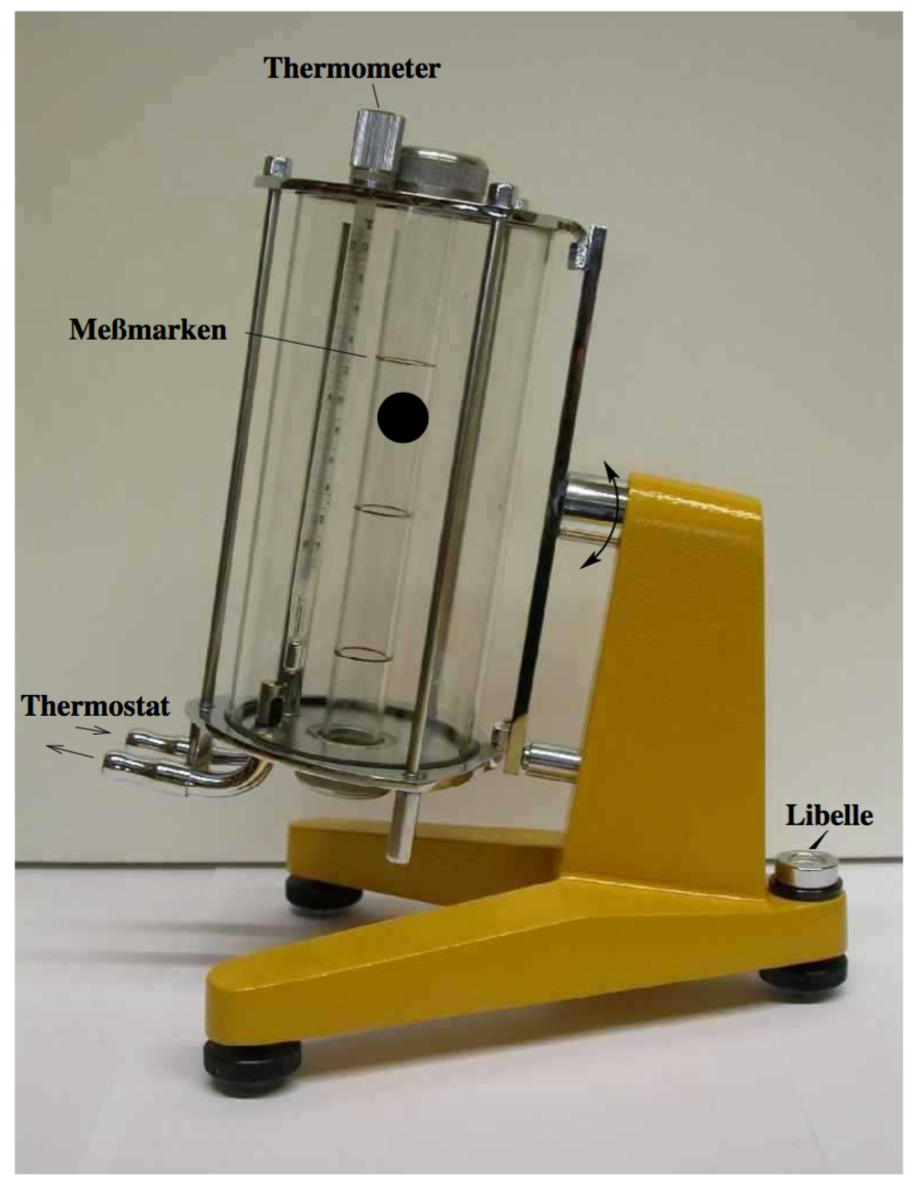
\includegraphics[height = 10 cm]{hoepplervisko.pdf}
  \caption{Das Höppler-Viskosimeter\cite{anleitung}.}
  \label{fig:hoeppvisko}
\end{figure}

Damit die benutzte Glaskugel nicht unkontrolliert gegen die Wände schlägt,
ist das Fallrohr leicht geneigt. Die Temperatur des Fallrohrs kann durch ein
Thermostat geregelt werden, dass das Wasserbad erhitzt von dem das Fallrohr
umgeben ist. Die Messmarken markieren eine feste Messstrecke.

Die Messungen werden mit einer kleinen und einer großen Glaskugel bestimmt,
dessen Radius sich aber nur geringfügig unterscheidet.
\begin{enumerate}
  \item Zunächst wird die Dichte der beiden Kugeln durch Messen der Masse
  und des Duchmessers bestimmt. Um eine Angabe über die Genauigkeit zu erhalten
  wird der Durchmesser vier Mal gemessen. Die Masse wird nur ein Mal bestimmt.

  \item Dann wird das Fallrohr mit destilliertem Wasser und einer der
  Glaskugeln befüllt und es werden möglichst
  alle Luftblasen entfernt.

  \item Nach Verschließen der Schrauben wird das Fallrohr gedreht und
  die Fallzeit der Strecke $\SI{100}{\milli\meter}$ gleichzeitig mit zwei
  Stoppuhren gemessen, sodass nach fünf Durchgängen zehn Messwerte aufgenommen
  werden konnten. Diese Messung wird zunächst mit der kleinen Kugel durchgeführt.
  Dann kann mit der gegebenen Apparatekonstante $K_{\text{kl}} = \SI{0.07640}
  {\milli\pascal\cubic\centi\meter\per\gram}$ die Viskosität bestimmt werden.
  Nach weiteren fünf Durchgängen mit der großen Kugel
   kann durch Umstellen der Gleichung \eqref{eqn:visko1} die
  Apparatekonstante $K_{\text{gr}}$ bestimmt werden.

  \item Um die Konstanten $\symup{A}$ und $\symup{B}$ aus Gleichung
  \eqref{eqn:andra} zu bestimmen wird das destillierte Wasser auf
  $\SI{70}{\celsius}$ erhitzt und bei 10 Temperaturen jeweils zwei Mal
  die Fallzeit gemessen.


\end{enumerate}

\newpage
